\begin{wrapfigure}{r}{0.5\textwidth}
    \vspace{-1.5em}
    \centering
    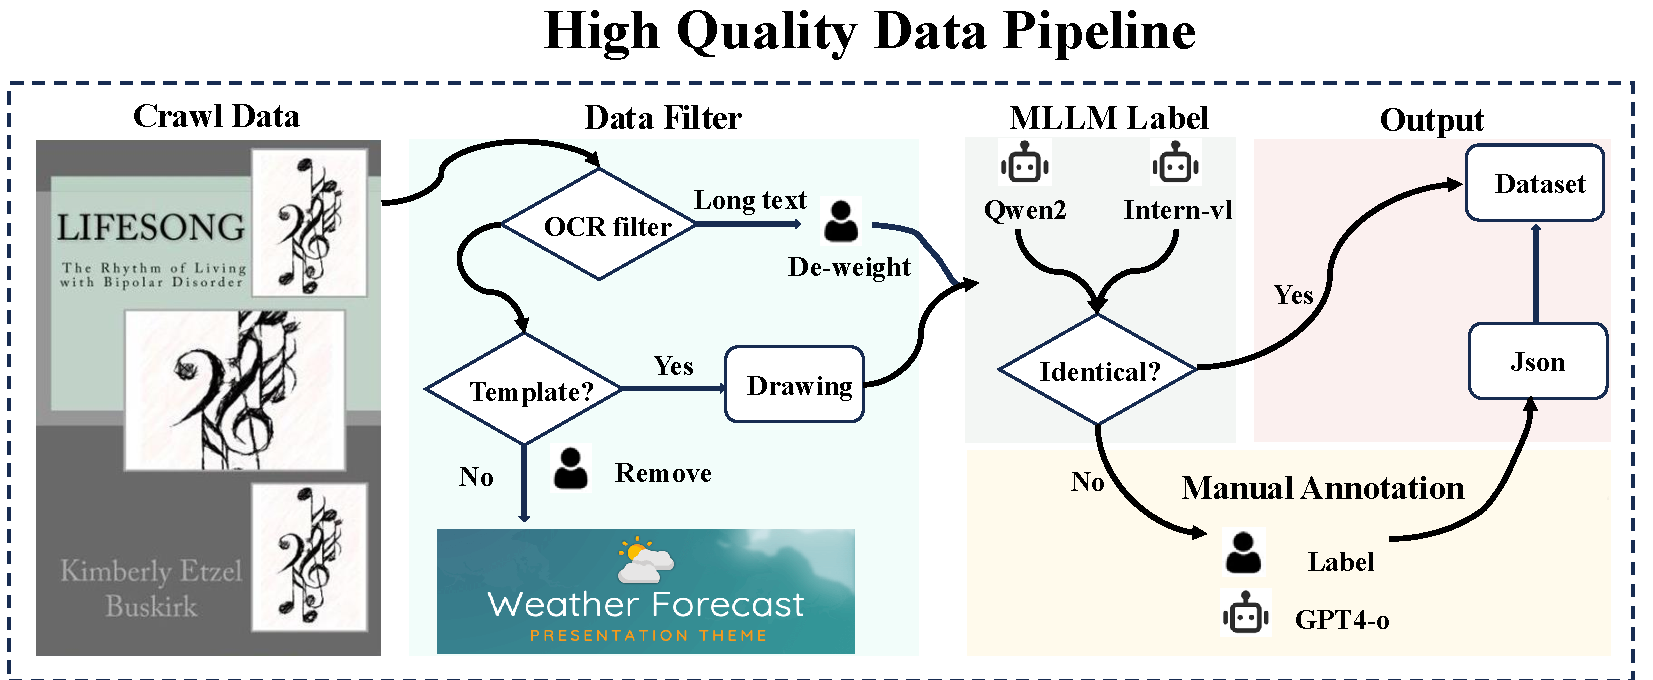
\includegraphics[width=0.48\textwidth]{figures/src/hqpipeline_fig4.pdf}
    % \vspace{-1.5em}
    \caption{
    \textbf{TextScenesHQ Generation Pipeline.}
    Data is filtered using OCR  and refined manually to correct inconsistencies from VLM.
    }
    \label{fig:high_quality_ppl}
    \vspace{-1.5em}
\end{wrapfigure}


% \begin{figure}
%     \centering
%     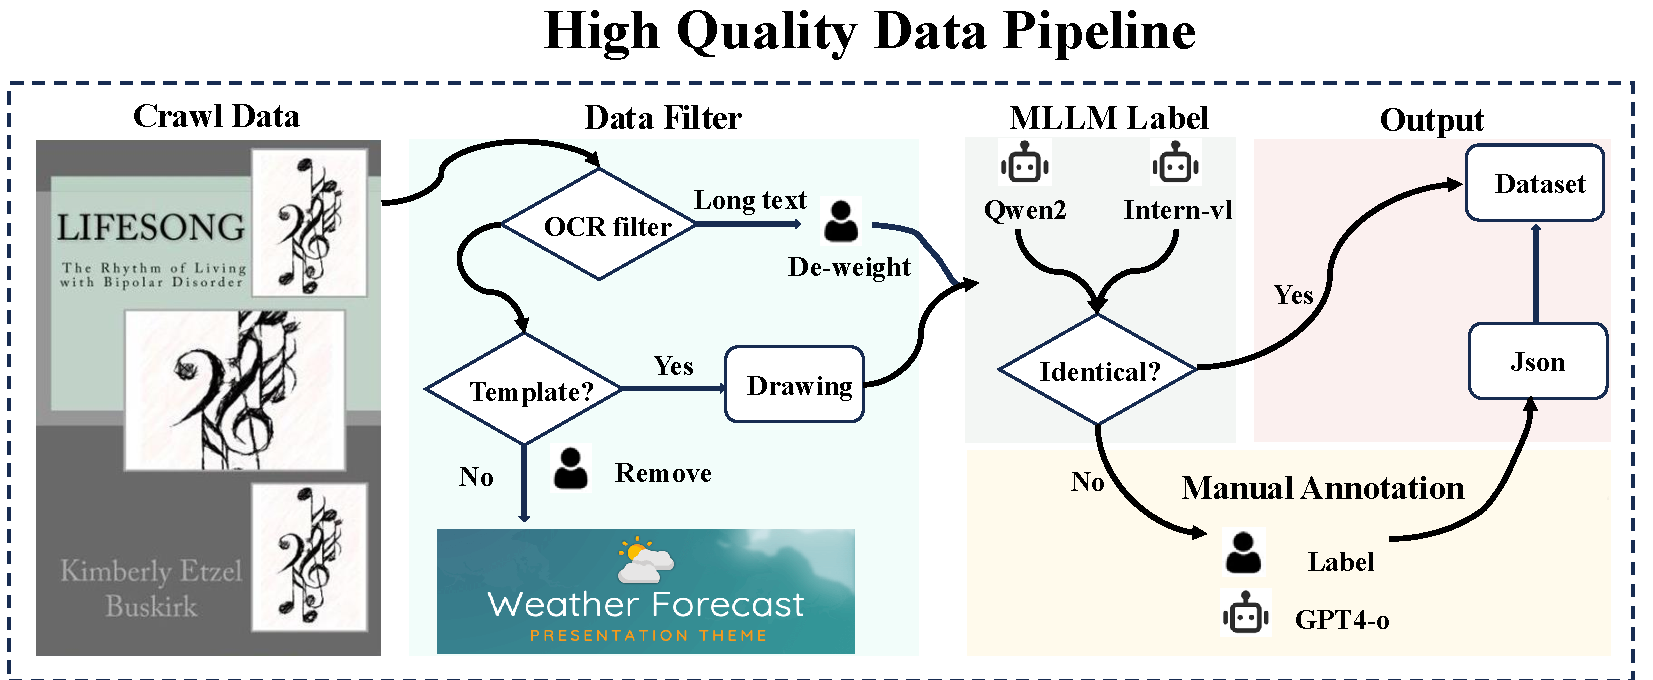
\includegraphics[width=.85\linewidth]{figures/src/hqpipeline_fig4.pdf}
%     \caption{
%     \textbf{TextScensHQ Generation Pipeline.}
%     The data is filtered using OCR results and manual annotation with correcting inconsistencies from vision-language models.
%     % The raw data undergoes rigorous filtering based on OCR rules to ensure quality. Additionally, manual annotation is applied to address inconsistencies in annotations from existing large-scale vision-language models.
%     }
%     \label{fig:high_quality_ppl}
% \end{figure}